\documentclass[10pt]{article}
\usepackage[usenames]{color} %used for font color
\usepackage{amssymb} %maths
\usepackage{amsmath} %maths
\usepackage[utf8]{inputenc} %useful to type directly diacritic characters
\usepackage{tikz}
\usepackage{pgfplots}
\usepackage{tikz-3dplot}
\usepackage{chemfig}
\usetikzlibrary{calc,math}
\usepgfplotslibrary{groupplots}

\begin{document}

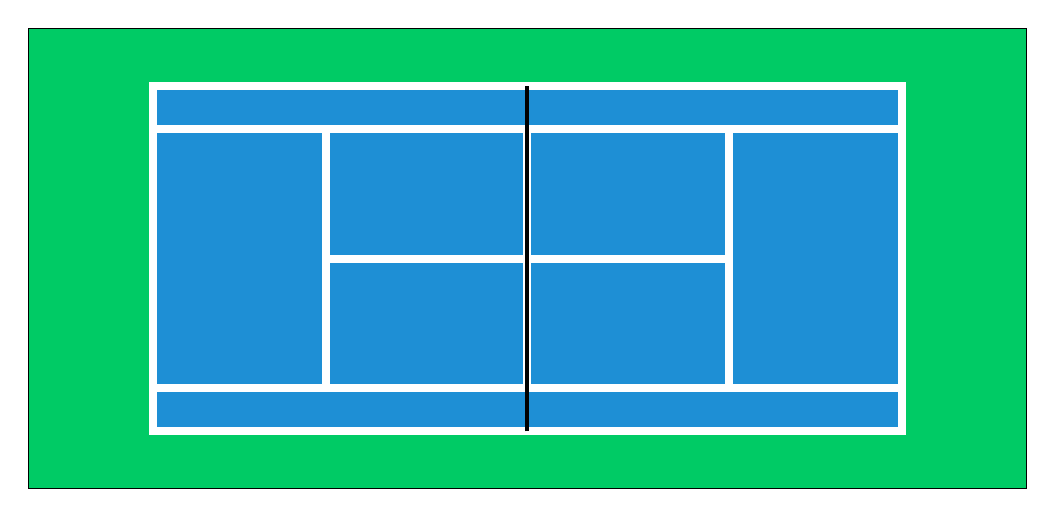
\begin{tikzpicture}[scale=0.4]
   \definecolor{tennisblue}{rgb}{0.1176,0.5608,0.8353}
    \definecolor{tennisgreen}{rgb}{0,0.797,0.398}

    % Court dimensions
    \def\courtWidth{10.97}
    \def\courtLength{23.77}
    \def\baselineLength{8.23}
    \def\netHeight{0.914}
    \def\singlesWidth{8.23}
    \def\serviceLength{6.4}


    % Draw court outline
    \draw[fill=tennisgreen] (-\courtLength/1.5, -\courtWidth/1.5) rectangle (\courtLength/1.5, \courtWidth/1.5);
    \draw[fill=tennisblue] (-\courtLength/2, -\courtWidth/2) rectangle (\courtLength/2, \courtWidth/2);
    \draw[line width = 0.1cm, white] (-\courtLength/2, -\courtWidth/2) rectangle (\courtLength/2, \courtWidth/2);


    % Draw service boxes
    \draw[line width = 0.1cm, white] (0, 0) rectangle (- \serviceLength, \singlesWidth/2);
    \draw[line width = 0.1cm, white] (0, 0) rectangle (\serviceLength, \singlesWidth/2);
    \draw[line width = 0.1cm, white] (0, 0) rectangle (\serviceLength, -\singlesWidth/2);
    \draw[line width = 0.1cm, white] (0, 0) rectangle (-\serviceLength, -\singlesWidth/2);

    \draw[line width = 0.1cm, white] (-\serviceLength, -\singlesWidth/2) -- (-\courtLength/2, -\singlesWidth/2);
    \draw[line width = 0.1cm, white] (\serviceLength, -\singlesWidth/2) -- (\courtLength/2, -\singlesWidth/2);
    \draw[line width = 0.1cm, white] (\serviceLength, \singlesWidth/2) -- (\courtLength/2,\singlesWidth/2);
    \draw[line width = 0.1cm, white] (-\serviceLength, \singlesWidth/2) -- (-\courtLength/2,\singlesWidth/2);

    % Draw center mark
    \draw[line width = 0.05cm, black] (0, -\courtWidth/2) -- (0, \courtWidth/2);


\end{tikzpicture}


\end{document}